\documentclass[10pt,landscape]{article}
\usepackage{multicol}
\usepackage{calc}
\usepackage{ifthen}
\usepackage[landscape]{geometry}
\usepackage[hidelinks]{hyperref}
\usepackage{graphicx}
\usepackage[export]{adjustbox}
\usepackage{enumitem}

\usepackage[defaultsans]{droidsans}
\renewcommand*\familydefault{\sfdefault} %% Only if the base font of the document is to be typewriter style
\usepackage[T1]{fontenc}


\usepackage{listings}
\usepackage{color}

\definecolor{codegreen}{rgb}{0,0.6,0}
\definecolor{codegray}{rgb}{0.5,0.5,0.5}
\definecolor{codepurple}{rgb}{0.58,0,0.82}
\definecolor{backcolour}{rgb}{0.95,0.95,0.95}
\definecolor{lightgrey}{gray}{0.6}

\lstdefinestyle{definitioncode}{
    backgroundcolor=\color{backcolour},
    commentstyle=\color{codegreen},
    keywordstyle=\color{magenta},
    numberstyle=\tiny\color{codegray},
    stringstyle=\color{codepurple},
    basicstyle=\footnotesize,
    breakatwhitespace=false,
    breaklines=true,
    captionpos=b,
    keepspaces=true,
    numbers=none,
    numbersep=5pt,
    showspaces=false,
    showstringspaces=false,
    showtabs=false,
    tabsize=2
}
\lstdefinestyle{examplecode}{
    backgroundcolor=,%
    numberstyle=\tiny\color{codegray},
    stringstyle=\color{codepurple},
    basicstyle=\footnotesize,
    breakatwhitespace=false,
    breaklines=true,
    captionpos=b,
    keepspaces=true,
    numbers=none,
    numbersep=5pt,
    showspaces=false,
    showstringspaces=false,
    showtabs=false,
    tabsize=2
}


\lstset{style=definitioncode}



% This sets page margins to .5 inch if using letter paper, and to 1cm
% if using A4 paper. (This probably isn't strictly necessary.)
% If using another size paper, use default 1cm margins.
\ifthenelse{\lengthtest { \paperwidth = 11in}}
{ \geometry{top=.5in,left=.5in,right=.5in,bottom=.5in} }
{\ifthenelse{ \lengthtest{ \paperwidth = 297mm}}
    {\geometry{top=1cm,left=1cm,right=1cm,bottom=1cm} }
    {\geometry{top=1cm,left=1cm,right=1cm,bottom=1cm} }
}

% Turn off header and footer
\pagestyle{empty}


% Redefine section commands to use less space
\makeatletter
\renewcommand{\section}{\@startsection{section}{1}{0mm}%
                                {-1ex plus -.5ex minus -.2ex}%
                                {0.5ex plus .2ex}%x
                                {\normalfont\large\bfseries}}
\renewcommand{\subsection}{\@startsection{subsection}{2}{0mm}%
                                {-1explus -.5ex minus -.2ex}%
                                {0.5ex plus .2ex}%
                                {\normalfont\normalsize\bfseries}}
\renewcommand{\subsubsection}{\@startsection{subsubsection}{3}{0mm}%
                                {-1ex plus -.5ex minus -.2ex}%
                                {1ex plus .2ex}%
                                {\normalfont\small\bfseries}}
\makeatother

% Define BibTeX command
\def\BibTeX{{\rm B\kern-.05em{\sc i\kern-.025em b}\kern-.08em
    T\kern-.1667em\lower.7ex\hbox{E}\kern-.125emX}}

% Don't print section numbers
\setcounter{secnumdepth}{0}


\setlength{\parindent}{0pt}
\setlength{\parskip}{0pt plus 0.5ex}


% -----------------------------------------------------------------------

\begin{document}

\raggedright
\footnotesize
\begin{multicols}{3}


% multicol parameters
% These lengths are set only within the two main columns
%\setlength{\columnseprule}{0.25pt}
\setlength{\premulticols}{1pt}
\setlength{\postmulticols}{1pt}
\setlength{\multicolsep}{1em}
\setlength{\columnsep}{1em}

\includegraphics[width=2cm,valign=t]{res/yadtlogo}%
\hfill%
\begin{minipage}[t]{5cm}
{\Large{\textbf{yadt 1.8}}}\hfill
\textcolor{lightgrey}{cheat sheet 0.3}\\[1em]
~\hfill\href{http://www.yadt-project.org/}{http://www.yadt-project.org/}
\end{minipage}


\section{Concept}
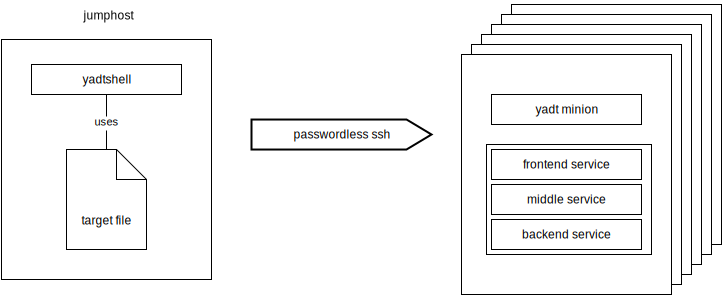
\includegraphics[width=\linewidth]{res/concept}

Using the yadtshell you can execute high level operations like updating
a group of hosts . The only requirement is that the hosts are accessible
via passwordless ssh and provide a yadt client.



\section{Definition: Component URI}

\begin{lstlisting}
host://<hostname>
service://<hostname>/<name>
artefact://<hostname>/<name>/<version>
\end{lstlisting}

\emph{Examples}
\begin{lstlisting}[style=examplecode]
host://hostname
service://hostname/tomcat6
artefact://hostname/web-application/0:1.23
\end{lstlisting}

Components are \emph{always} host-specific.

\subsection{Brace Exception}
\begin{lstlisting}
artefact://{hostname01|hostname03}/myapp
\end{lstlisting}

\subsection{Range Expression}
\begin{lstlisting}
host://hostname0[1..3]
\end{lstlisting}

\subsection{Wildcards}
\begin{lstlisting}
service://hostname/*
\end{lstlisting}



\section{yadt.conf.d (directory)}

The yadt minion gets configured via *.yaml files in /etc/yadt.conf.d;
they get merged in alphanumeric order.
\\
\emph{Keep in mind}: Indented blocks have to start with \emph{4 blanks}. 
Do not use tabs.

\begin{lstlisting}[showspaces=true]
services:
    frontend:
        needs_services: [middleservice1]
        is_frontservice: true
    middleservice1:
        needs_services: [middleservice2]
\end{lstlisting}

The service name must be equal to the corresponding name of the
service script (as found in /etc/init.d).

\begin{description}[font=\bfseries,leftmargin=1cm,style=sameline]
    \item [is\_frontservice]
    is a marker for the status overview. The status
    (shown in percentage) of the target will be
    calculated by determining how many
    frontservices are running.
\item [needs\_services]
    the services that have to be running before
    starting this service (reverse for stopping)
\end{description}

The service definition may contain a component URI as string,
which describes a service on another host, e.g.

\begin{lstlisting}
needs_services: ['service://hostname/servicename']
\end{lstlisting}

Please note that this notation only allows the \emph{hostname},
not the full qualified domain name. Yadtshell extracts the hostname from
the fqdn as the string until the first dot.

Please see the \emph{Merging configuration} section for more information.



\section{target (file)}

yadtshell uses a yaml file named target in the current working directory to define a yadt target (set of hosts), e.g.

\begin{lstlisting}
hosts:
- hostname1.spam.eggs
- hostname2.spam.eggs
- hostname*.spammy.eggs
- hostname0[1..3].foo.bar
\end{lstlisting}

It is possible to group your hosts within a target:

\begin{lstlisting}
hosts:
- hostname1.spam.eggs hostname2.spam.eggs
- hostname3.foo.bar hostname4.foo.bar
\end{lstlisting}

this will change the way the hosts will be displayed.



\section{view (file)}

If you have a lot of hosts in a target you can use a yaml-file
called view to configure the rendering of the status overview.
Place the view file together with the target file in the current
working directory.

\begin{lstlisting}
info-view: [matrix, color]
\end{lstlisting}

\begin{description}[font=\bfseries,leftmargin=1.5cm,style=sameline]
    \item [matrix]  show status information in matrix
    \item[color]    display status in color
    \item[maxcols]  maximum number of columns
    \item[3cols]    use three columns
\end{description}



\vfill\columnbreak



\section{Executing yadt commands}

All involved hosts have to be accessible via \emph{passwordless ssh}.


\subsection{1. Entering the yadtshell}

Enter the yadtshell by calling
\begin{lstlisting}
init-yadtshell
\end{lstlisting}

\begin{itemize}
\item activates autocompletion for component uris,
\item allows to omit \verb#yadtshell# when executing a yadtshell commands.
\end{itemize}

To restores your shell environment you can use \verb#CTRL+D# or

\begin{lstlisting}
deactivate
\end{lstlisting}


\subsection{2. Using yadtshell as a command}

Use the \verb#yadtshell# command if you prefer to execute yadtshell commands
without entering the yadtshell itself:
\begin{lstlisting}
yadtshell [options] <command> [<uri> ...]
\end{lstlisting}

\begin{description}[font=\bfseries,leftmargin=1.5cm,style=sameline]
    \item [-v]       verbose
    \item [--dryrun] no actions executed (just logging)
    \item [-n]       same as dryrun
\end{description}



\subsection{Status Information}

To retrieve the status of all services and artefacts versions from the current
target use:
\begin{lstlisting}
status
\end{lstlisting}

this will also perform \verb+info+, which displays a summary of all
services for each host within the current target:
\begin{lstlisting}
info [--full]
\end{lstlisting}

\begin{description}[font=\bfseries,leftmargin=1.5cm,style=sameline]
    \item [--full]     shows complete information (artefacts of hosts, etc.)
\end{description}

To display low-level data of components (in yaml format) use
\begin{lstlisting}
dump [uri-query0 [uri-query1 ...]]
\end{lstlisting}

additional arguments for \verb+dump+:
\begin{description}[font=\bfseries,leftmargin=1.5cm,style=sameline]
    \item [--attribute]
    \item [--show-pending-updates]
    \item [--show-current-artefacts]
\end{description}

\emph{Example:} dump info of all services.
\begin{lstlisting}
dump service://
\end{lstlisting}

\emph{Note: The output of info and dump is generated using cached data.}



\vfill\columnbreak
\subsection{Hosts}

To prevent others from executing commands on a host it is possible to lock the host:
\begin{lstlisting}
lock -m "message" [--force] <host_uri> [<host_uri> ...]
\end{lstlisting}

afterwards commands can only be executed
\begin{itemize}
\item by you,
\item from the current target directory
\item on the current host.
\end{itemize}

\emph{Example:} lock the host \verb+hostname01+
\begin{lstlisting}
lock -m "message" host://hostname01
\end{lstlisting}

\emph{Example:} hijacking a lock from somebody else
\begin{lstlisting}
lock -m "message" --force host://*
\end{lstlisting}

\emph{Attention:} when using the \verb+-m "message"+ option, the message
should reflect the reason why you are doing what you are doing and
include your name as well:
\begin{lstlisting}
lock -m "Need this host. [Michael]" host://hostname31
\end{lstlisting}

To release a lock use:
\begin{lstlisting}
unlock <host_uri> [<host_uri] ...]
\end{lstlisting}

\emph{Example:} release all of your locks on all target hosts.
\begin{lstlisting}
unlock host://*
\end{lstlisting}



\vfill\columnbreak
\subsection{Services}

To start a service, regarding its dependencies, use:
\begin{lstlisting}
start <service_uri> [<service_uri> ...]
\end{lstlisting}

\emph{Example:} start all services.
\begin{lstlisting}
start service://*
\end{lstlisting}

To stop a service and all services depending on the service:
\begin{lstlisting}
stop <service_uri> [<service_uri> ...]
\end{lstlisting}

\emph{Keep in mind:} When stopping a service all services depending on this service will be
stopped as well. But starting the service will \emph{not} start the services
depending on the service again.


If a service is currently out of order you can ignore the state of a service
(e.g. assume all operations on that service are successful):
\begin{lstlisting}
ignore -m "message" <service_uri> [<service_uri> ...]
\end{lstlisting}

\emph{Example:} ignore all nagios checks, since the nagios server is down
\begin{lstlisting}
ignore -m "nagios server is down" service://*/nagios
\end{lstlisting}

To unignore services on host use:
\begin{lstlisting}
unignore <service_uri> [<service_uri> ...]
\end{lstlisting}



\vfill\columnbreak
\subsection{Artefacts}

To install updates (if there are any) and stop/start the defined services use:
\begin{lstlisting}
update <host_uri> [<host_uri> …] [-p <number>]
\end{lstlisting}

If you only want to update artefacts without restarting services,
use \verb+updateartefact+. Take care when using this command:
it is ignoring all service dependencies.
\begin{lstlisting}
updateartefact <artefact_uri> [...]
\end{lstlisting}



\scriptsize
\hfill\href{http://www.yadt-project.org/}{http://www.yadt-project.org/}
\includegraphics[width=2cm]{res/yadtlogo}

\end{multicols}
\end{document}
